\newlecture{4}{Graphs, Tables and Code}

\section{Graphs}

\subsection{Include Graphs}

\begin{frame}[fragile]{Include Graphs}
Before all, you need the \packagename{graphics} or \packagename{graphicx} package, where \packagename{graphicx} is an extended and enhanced one. So you are recommended to insert the command in the preamble of your document.

\begin{command}
\LC|\usepackage{graphicx}|
\end{command}

Then you can use the command \LC|\includegraphics| to insert images of many formats, including \packagename{jpg}, \packagename{png} images and even other \packagename{pdf} files. \packagename{eps} images should be supported by most modern \LaTeX\ distributions as well.

\begin{command}
\LC|\includegraphics[options]{filename}|
\end{command}

\end{frame}

\begin{frame}[fragile]
There are some example images defined, you can insert them if the figure is not yet ready when writing \LaTeX\ code. They are \packagename{example-image}, \packagename{example-image-golden}, \packagename{example-image-a}, \packagename{example-image-b} and etc.

\begin{latexexample}
\includegraphics[width=0.4\textwidth]{example-image}
\end{latexexample}

We usually use the \packagename{width} option to adjust the size of the image, according to a ratio of \LC|\textwidth|, which means the maximum width of text here.

\end{frame}


\begin{frame}[fragile]{Options of Include Graphs}
	Here some useful \packagename{options} are listed:
	\begin{itemize}
		\item \packagename{height} - use any \LaTeX\ measuring unit.
		\item \packagename{width} - use any \LaTeX\ measuring unit.
		\item \packagename{scale} - scale the graph to this proportion
		\item \packagename{angle} - rotate the graph in anti-clockwise by this angle 
	\end{itemize}
	
	\LaTeX\ measuring unit can be \LC|\textwidth|, \LC|\linewidth|, \LC|\textheight|, \LC|\lineheight|, cm, pt, em, and etc..

\begin{latexexamplesplit}
\includegraphics[width=4cm]%
{example-image-a}
\end{latexexamplesplit}

%	\begin{minipage}{0.5\linewidth}
%		\begin{example}
%\begin{minted}{latex}
%\usepackage{graphicx}
%\begin{figure}[htbp]
%    \centering
%    \includegraphics[width=0.5 \linewidth]{sample.jpg}
%    \caption{Marshmallow}
%    \label{fig-sample}
%\end{figure}
%\end{minted}
%		\end{example}
%	\end{minipage}
%	\hfill
%	\begin{minipage}{0.45\linewidth}
%		\begin{figure}[htbp]
%			\centering
%			\includegraphics[width=0.5\linewidth,angle=180]{sample.jpg}
%			\caption{Marshmallow}
%			\label{fig-sample}		
%		\end{figure}
%	\end{minipage}
\end{frame}

\subsection{Figures}

\begin{frame}[fragile]{The \packagename{figure} Environment}
	The \packagename{figure} environment provides a wrapper of image inserted by \LC|\includegraphics|, which add caption and label (reference) to an image. They are especially useful in report and paper writing, here is a template of how to use the environment.

\begin{command}
\begin{LCL}
\begin{figure}[position]
  \centering
  \includegraphics[options]{filename}
  \caption{caption}
  \label{fig:label}
\end{figure}
\end{LCL}
\end{command}
	
\begin{itemize}
			\item \packagename{filename} - the filename or relative path of the graph you want to insert, usually placed in the same or child directory as the tex file
			\item \packagename{position} - we usually use \packagename{!htbp} or \packagename{!H} here, which will be introduced later in this chapter
			\item \packagename{caption} - the caption displayed above/under the graph
			\item \packagename{label} - used for references in a document (will be introduced later)
\end{itemize}

\end{frame}

\begin{frame}[fragile]{Labels and References}

You can use \LC|\ref| to have a reference of a figure by its label. The figures will be automatically numbered (like equations), and the reference is also a hyperlink.

\begin{latexexamplesplit}[0.6]
\begin{figure}[!htbp]
  \centering
  \includegraphics[
    width=0.8\textwidth,
    angle=90
  ]{example-image-b}
  \caption{Example Image B rotated by 90 degree.}
  \label{fig:img-b}
\end{figure}
B was shown in Figure
\ref{fig:img-b}.
\end{latexexamplesplit}


\end{frame}

\begin{frame}[fragile]{Floats and Positions}

Floats are containers for things in a document that cannot be broken over a page. \LaTeX\ by default recognizes \packagename{figure} and \packagename{table} (will be introduced later) floats. \medskip

If you don't provide the \packagename{position} option, \LaTeX\ will try to help you find a place to set the figure. However, the position is often not ideal, so you need to add some specifiers yourselves. 

\begin{itemize}
\item \packagename{h} - Place the float \structure{here}, i.e., approximately at the same point it occurs in the source text (however, not exactly at the spot)
\item \packagename{t} - Position at the \structure{top} of the page.
\item \packagename{b} - Position at the \structure{bottom} of the page.
\item \packagename{p} - Put on a special \structure{page} for floats only.
\item \packagename{!} - Override internal parameters \LaTeX\ uses for determining ``good'' float positions.
\item \packagename{H} -  Places the float at precisely the location in the \LaTeX\ code. Requires the float package, i.e., \LC|\usepackage{float}|.
\end{itemize}

\end{frame}


%\begin{frame}[fragile]
%	Usually you need to optimize the size and some other properties of the graph, most of them can be set in \structure{options}. (Only some useful options are listed here)
%	\begin{itemize}
%		\item \structure{height} - use any \LaTeX\ measuring unit.
%		\item \structure{width} - use any \LaTeX\ measuring unit.
%		\item \structure{scale} - scale the graph to this proportion
%		\item \structure{angle} - rotate the graph in anti-clockwise by this angle 
%	\end{itemize}
%	\begin{minipage}{0.5\linewidth}
%		\begin{example}
%\begin{minted}{latex}
%\usepackage{graphicx}
%\begin{figure}[htbp]
%    \centering
%    \includegraphics[width=0.5 \linewidth]{sample.jpg}
%    \caption{Marshmallow}
%    \label{fig-sample}
%\end{figure}
%\end{minted}
%		\end{example}
%	\end{minipage}
%	\hfill
%	\begin{minipage}{0.45\linewidth}
%		\begin{figure}[htbp]
%			\centering
%			\includegraphics[width=0.5\linewidth,angle=180]{sample.jpg}
%			\caption{Marshmallow}
%			\label{fig-sample}		
%		\end{figure}
%	\end{minipage}
%\end{frame}


%\begin{frame}[fragile]{}
%\begin{multicols}{2}

%\begin{figure}[H]
%  \centering
%  \includegraphics[width=0.2\textwidth]{example-image-a}
%  \caption{caption}
%  \label{figure-label}
%\end{figure}
%
%Some test
%
%Some other text
%\end{multicols}
%
%\end{frame}


\begin{frame}[fragile]{Include Multiple Graphs}
    A useful extension is the \packagename{subcaption} package, which provides a \packagename{subfigure} environment to add multiple subfigures in a figure. \medskip
    
    Note that there is also a package called 	\packagename{subfigure}, but is has been deprecated (not maintained), please do not use it. Another package called \packagename{subfig} provides the same commands as that of \packagename{subfigure} package. However, they can't be used together. \medskip
    
    In simplicity, if there is some compatibility problem with your template after you tried the \packagename{subcaption} package, choose the \packagename{subfig} package. \medskip
    
    Here is an example with the \packagename{subcaption} package.
\end{frame}

\begin{latexexampleframe}
\begin{figure}
    \centering
    \begin{subfigure}{0.3\textwidth}
        \includegraphics[width=\textwidth]{example-image-a}
        \caption{Example Image A.}
        \label{fig:subcaption-a}
    \end{subfigure}
    ~ 
    \begin{subfigure}{0.3\textwidth}
        \includegraphics[width=\textwidth]{example-image-b}
        \caption{Example Image B.}
        \label{fig:subcaption-b}
    \end{subfigure}
    
    \begin{subfigure}{0.3\textwidth}
        \includegraphics[width=\textwidth]{example-image-c}
        \caption{Example Image C.}
        \label{fig:subcaption-c}
    \end{subfigure}
    \caption{Example Images}\label{fig:subcaption}
\end{figure}
\end{latexexampleframe}

\begin{frame}[fragile]
  
As shown in Figure \ref{fig:subcaption}, the figures can be arranged in columns and rows. \medskip

Between Figure \ref{fig:subcaption-a} and Figure \ref{fig:subcaption-b}, a \LC|~| was added. You can add desired spacing between images, e. g. \LC|~|, \LC|\quad|, \LC|\qquad|, \LC|\hfill| (fill all rest horizontal spaces) and etc.. \medskip

Between Figure \ref{fig:subcaption-b} and Figure \ref{fig:subcaption-c}, a newline was added. It will force the subfigure onto a new line. \medskip

The references of subfigures can be used by their \LC|\label| as well. For example, above references are generated by these commands:
\begin{example}
\begin{LCL}
\ref{fig:subcaption}
\ref{fig:subcaption-a}
\ref{fig:subcaption-b}
\ref{fig:subcaption-c}
\end{LCL}
\end{example}

\end{frame}

\subsection{Draw Graphs}

\begin{frame}[fragile]{The \packagename{tikz} and \packagename{pgf} packages}

The \packagename{tikz} and \packagename{pgf} packages can help you draw graphs in \LaTeX\, for example:

\begin{example}
\inputminted{latex}{../examples/relation.tex}
\end{example}

\end{frame}

\begin{frame}

This will generate a simple graph which consists of eight nodes:
\begin{center}
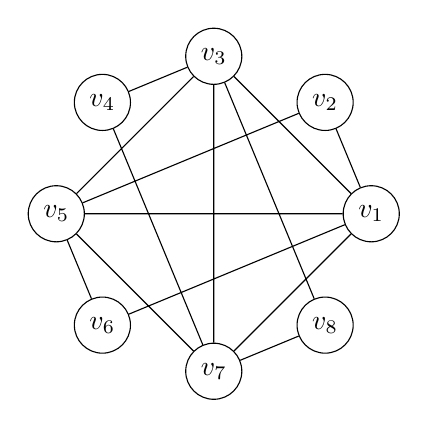
\begin{tikzpicture}[scale=2, bend angle=22.5]
\tikzstyle{every node}=[draw,shape=circle];
\foreach \i in {1,...,8}
{
\path (45*\i-45:1cm) node (v\i) {$v_\i$};
}
\draw
(v1) -- (v2) (v3) -- (v4) (v5) -- (v6) (v7) -- (v8)
(v1) -- (v3) (v3) -- (v5) (v5) -- (v7) (v7) -- (v1)
(v2) -- (v5) (v4) -- (v7) (v6) -- (v1) (v8) -- (v3)
(v1) -- (v5) (v3) -- (v7);
\end{tikzpicture}
\end{center}

There may be a lecture about \packagename{tikz} and \packagename{pgf} in the future. If you are now interested in it, please refer to the \structure{pgf manuel} by \mintinline{shell}|texdoc tikz| or \mintinline{shell}|texdoc pgf|.

\end{frame}

\begin{frame}[fragile]

Another example:

\begin{example}
\inputminted[firstline=1,lastline=20]{latex}{../examples/binary_tree.tex}
\end{example}

\end{frame}

\begin{frame}

\begin{exampleblock}{}
\inputminted[firstline=21]{latex}{../examples/binary_tree.tex}
\end{exampleblock}

This will generate a binary tree:
\begin{center}
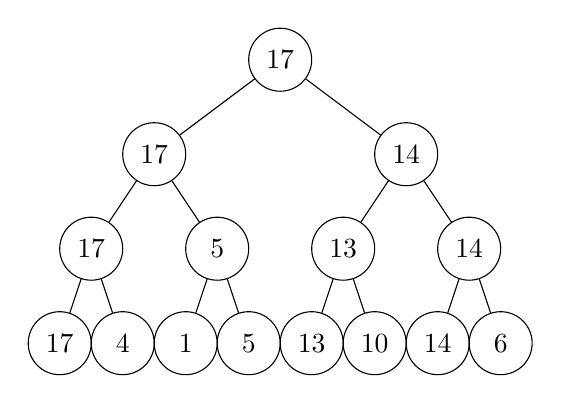
\begin{tikzpicture}[scale=0.8]
\tikzstyle{every node}=[draw,shape=circle,minimum size=0.8cm];
\node {17}[sibling distance=4cm]
child { node {17}[sibling distance=2cm]
	child {
		node {17}[sibling distance=1cm]
		child { node {17} }
		child { node {4} }
	}
	child {
		node {5}[sibling distance=1cm]
		child { node {1} }
		child { node {5} }
	}
}
child { node {14}[sibling distance=2cm]
	child {
		node {13}[sibling distance=1cm]
		child { node {13} }
		child { node {10} }
	}
	child {
		node {14}[sibling distance=1cm]
		child { node {14} }
		child { node {6} }
	}
};
\end{tikzpicture}
\end{center}

\end{frame}


\section{Tables}

\subsection{Tabulars}

\begin{frame}[fragile]{The \packagename{tabular} Environment}
	Table is another common element in \LaTeX, usually you will need the \packagename{array} package for enhanced functions of tables. You can insert the command in the preamble of your document.

\begin{command}
\LC|\usepackage{array}|
\end{command}

\begin{latexexamplesplit}
\begin{tabular}{|l|c|r|}
  \hline
  Title 1 & Title 2 & Title 3 \\
  \hline
  1 & 2 & 3 \\
  \hline
\end{tabular}
\end{latexexamplesplit}

The syntax is similar to the \packagename{align} environment in maths. \LC|&| is used to split the columns are \LC|\\| is used to split the rows. \medskip

%\LC|\hline| is used to draw the horizontal lines in the table.


\end{frame}

\begin{frame}[fragile]{Column Format}

\begin{command}
\begin{LCL}
\begin{tabular}{format}
...
\end{tabular}
\end{LCL}
\end{command}

	\packagename{format} can be set as follow:
	\begin{itemize}
		\item \packagename{|} - represents a vertical separate line between two columns
		\item \packagename{l} - align left in this column
		\item \packagename{c} - align center in this column
		\item \packagename{r} - align right in this column
	\end{itemize}
	\begin{example}
		\begin{minipage}{0.48\linewidth}
			\centering
			\packagename{|l|l|l|} \medskip
			
        	\begin{tabular}{|l|l|l|}
        		\hline
        		Title 1 & Title 2 & Title 3 \\
        		\hline
        		1 & 2 &3 \\
        		\hline
        	\end{tabular}
		\end{minipage}
		\begin{minipage}{0.48\linewidth}
			\centering
			\packagename{||c|cc||} \medskip
			
        	\begin{tabular}{||c|cc||}
        		\hline
        		Title 1 & Title 2 & Title 3 \\
        		\hline
        		1 & 2 &3 \\
        		\hline
        	\end{tabular}
		\end{minipage}
    \end{example}	
\end{frame}

\begin{frame}[fragile]

With the help of the \packagename{array} package, more formats are available:

\begin{itemize}
		\item \packagename{p\{width\}} - Equivalent to \LC|\parbox[t]{width}|, vertically aligned \alert{bottom}
		\item \packagename{b\{width\}} - Equivalent to \LC|\parbox[b]{width}|, vertically aligned \alert{top}
		\item \packagename{m\{width\}} - Equivalent to \LC|\parbox{width}|, vertically aligned middle
		\item \packagename{>\{decl.\}} - Can be used after a letter option, inserts \packagename{decl} before the entry.
		\item \packagename{<\{decl.\}} - Can be used before a letter option, inserts \packagename{decl} after the entry.
\end{itemize}

\packagename{t} and \packagename{b} may be very confusing, but that's how they work in \LC|\parbox|. With these new formats, the columns can be defined more flexibly.

\begin{latexexamplesplit}
\begin{tabular}
{|p{1.2cm}|b{1.2cm}|m{1.2cm}|}
  \hline
  Aligned Bottom & Aligned Top & 
  Aligned Middle \\
  \hline
  1 & 2 & 3 \\
  \hline
\end{tabular}
\end{latexexamplesplit}

\end{frame}

\begin{frame}[fragile]

\packagename{t}, \packagename{b} and \packagename{m} only affect the vertical alignment. If you want to control the width and make the text horizontally centered as well, you can use \LC|>{\centering}| to insert a \LC|\centering| before the text in that column. You can also insert \LC|>{$}| and \LC|<{$}| to generate a column in math mode.

\begin{latexexamplesplit}
\begin{tabular}{|>{\centering}m{2cm}|>{$}b{2cm}<{$}|}
  \hline
  Row of Text & 
  \text{Row of Maths} \\
  \hline
  First & x \\
  Second & x^2 \\
  \hline
\end{tabular}
\end{latexexamplesplit}

If a column type will be used many times, and also very long, you can define a new column type by yourselves. You can use 

\begin{command}
\LC|\newcolumntype{new type}{>{some declarations}{old type}<{some more declarations}}|
\end{command}

\end{frame}


\begin{frame}[fragile]

If you want to repeat a format for multiple times, you can use \LC|*{num}{format}|. Here's an example of the usage of \LC|\newcolumntype| with multiple columns form.

\begin{latexexamplesplit}
\newcolumntype{C}{>{$}c<{$}}
\newcolumntype{L}{>{$}l<{$}}
\newcolumntype{R}{>{$}r<{$}}

\begin{tabular}{|L| *{2}{C|} R|}
  \hline
  \text{First} & \text{Second} & 
  \text{Second} & \text{Third} \\
  \hline
  x & x^2 & x^2 & x^3 \\
  \hline
  y & y^2 & y^2 & y^3 \\
  \hline
\end{tabular}
\end{latexexamplesplit}

\end{frame}

\begin{frame}[fragile]{Horizontal Lines}

We usually need horizontal lines in tables. As shown in the examples above, you can add a \LC|\hline| at the beginning of a row. \medskip

If you only want to draw a partial line, use \LC|\cline[start-end]|.

\begin{latexexamplesplit}
\begin{tabular}{c|l|c|r}
  \hline\hline
  & Title 1 & Title 2 & Title 3 \\
  \cline{2-4}
  Table & 1 & 2 & 3 \\
  \cline{2-4}
  & 4 & 5 & 6 \\
  \hline\hline
\end{tabular}
\end{latexexamplesplit}


Here we draw a table with a multirow, but it only works with multirows of odd row number. A more convenient method of drawing multirows will be introduced.

\end{frame}

\begin{frame}[fragile]{Combine Rows and Columns}

There are two commands being used to combine rows and columns
\begin{command}
\LC|\multicolumn{ncols}{format}{text}|

\begin{itemize}
	\item \packagename{ncols} - the number of columns to be merged
	\item \packagename{format} - the format of the merged column, excluding the left \packagename{|} (eg. \packagename{c|})
	\item \packagename{text} - the text in the merged column
\end{itemize}

\LC|\multirow{nrows}{width}[fixup]{text}|

\begin{itemize}
	\item \packagename{nrows} - the number of rows to be merged
	\item \packagename{width} - the width of the merged rows (use \packagename{*} for auto)
	\item \packagename{fixup} - the vertical position of the text (optional, default in the center)
	\item \packagename{text} - the text in the merged row
\end{itemize}	

\end{command}

To use the \LC|\multirow| command, you need to insert the package \packagename{multirow} in the preamble of your document.

\end{frame}



\begin{frame}[fragile]

\begin{latexexample}
\centering
\begin{tabular}{|c|c|c|c|c|}
  \hline
  \multirow{4}{*}{Table} & Title 1 & Title 2 & Title 3 & Title 4 \\
  \cline{2-5}
  & \multicolumn{2}{c|}{Text 1} & 
  \multicolumn{2}{c|}{\multirow{3}{*}{Text 3}} \\
  \cline{2-3}
  & \multicolumn{2}{c|}{Text 2} & \multicolumn{2}{c|}{} \\
  \cline{2-3}
  & Text 4 & Text 5 & \multicolumn{2}{c|}{} \\
  \hline
\end{tabular}
\end{latexexample}

Just leave blank in the rest rows of \LC|\multirow|.

\end{frame}

\begin{frame}[fragile]{Table Generators}
	With \LC|\multirow| and \LC|\multicolumn|, we can almost draw tables of any style, but this coding process can never be as easy as the graphic one, like making tables in Word or Excel. Is there any ways to convert graphic tables into \LaTeX\ codes directly?\\
	\begin{itemize}
		\item Use \LaTeX\ Table Generator: \url{http://www.tablesgenerator.com/}
		\item \LaTeX\ Complex Table Editor: \url{https://www.latex-tables.com/}
		\item Excel2latex: \url{https://ctan.org/tex-archive/support/excel2latex/}
	\end{itemize}
\end{frame}

\subsection{Tables}

\begin{frame}[fragile]{The \packagename{table} Environment}

The \packagename{table} environment is used to arrange the place of a tabular, similar to the \packagename{figure} environment. Here is a template of how to use the environment.

\begin{command}
\begin{LCL}
\begin{table}[position]
  \centering
  \begin{tabular}{format}
    ...
  \end{tabular}
  \caption{caption}
  \label{table:label}
\end{table}
\end{LCL}
\end{command}

The \packagename{position}, \packagename{caption}, \packagename{label} are same as those in the \packagename{figure} environment. 
\end{frame}

\begin{frame}[fragile]{Recall the Positions}
	We usually want to place the graphs or tables just below or above the content where we mention them, but even when we type \packagename{[h]} in position, you can not ensure that it will appear at the ideal position, and there are several methods to make up for this. You can try them one by one: \medskip
	
	\begin{enumerate}
		\item Change \packagename{[h]} to \packagename{[!h]}
		\item Change \packagename{[!h]} to \packagename{[!H]}
		\item Use \LC|\newpage| to move the following content to the next page
	\end{enumerate}\medskip
	
Usually you don't need to pay too much attention about where the figures and tables are exactly are because you can use \LC|\ref| to reference them. And the numbering of 	figures and tables will strictly follow the order of their code.
	
\end{frame}

\begin{frame}[fragile]{\packagename{figure} and \packagename{table} in Two-column Documents}
If you are writing a document using two columns (i.e. you started your document with something like \LC|\documentclass[twocolumn]{article}|), you might have noticed that you can't use floating elements that are wider than the width of a column (using a \LaTeX\ notation, wider than \LC|0.5\textwidth|), otherwise you will see the figure or table overlapping with text. \medskip

If you really have to use such wide elements, the only solution is to use the ``starred'' variants of the floating environments:

\begin{command}
\begin{LCL}
\begin{figure*}[position]
  ...
\end{figure*}
\end{LCL}
\begin{LCL}
\begin{table*}[position]
  ...
\end{table*}
\end{LCL}
\end{command}

Those ``starred'' versions work like the standard ones, but they will be as wide as the page, so you will get no overlapping.

\end{frame}

\begin{frame}[fragile]{The \packagename{array} Environment}

	When you use \packagename{tabular} in maths environment, the text format in the \packagename{tabular} won't be italic. However, there is a replacement of \packagename{tabular}, which is the \packagename{array} environment.
	
\begin{command}
\begin{LCL}
\begin{array}{format}
  ...
\end{array}
\end{LCL}
\end{command}

The options and usages of these two environment are exactly the same. \medskip

Though the environment is not provided by the \packagename{array} package (it's built-in one), you are also recommended to use this package for enhancements.
	
\end{frame}

\subsection{Custom Floats}

\section{Code}

\subsection{Pseudo Code}

\subsection{Code Highlighting}

\begin{frame}[fragile]{The \packagename{minted} Package}

All of the code in this lecture are highlighted by the \packagename{minted} package. To use it, simply insert the command in the preamble of your document.

\begin{command}
\LC|\usepackage{minted}|
\end{command}

This is a very special package, it depends a program out of \LaTeX\, called \packagename{pygmentize}, which is a code highlighting package written in \packagename{Python}. \medskip

You can install the package through \packagename{pip} (assuming you have \packagename{Python} 2 or 3 and \packagename{pip} installed) in your terminal:

\begin{command}
\mintinline{shell}|pip install Pygments|
\end{command}

And then you can examine in your terminal whether \packagename{pygmentize} is your \packagename{PATH} by directly running it. You also need to add an option \packagename{-shell-escape} to your \LaTeX\ compiler because \LaTeX\ need this permission to run other programs on shell.

\end{frame}
